\section{Context of Use}
	Where there is code, there are bugs for sure. There are various tools and methods to test \& analyse the code before it goes into the real time environment. It is very fruitful if code analysis is done along with the traditional testing of the code, as it assists the enterprises to find the potential risks, vulnerabilities \& other weaknesses in the source code. If a vulnerability remains undetected it can cause a severe problem if its a multi-tiered system, as it will become a big deal to in both the aspects i.e time and budget. A well organised code analysis will prevent the enterprises from such troubles well before the time. ~\cite{C1}
	The traditional testing methods are not resilient enough to detect all the vulnerabilities and the threats in a multi-tiered or multiple tech infrastructures. If enterprises only rely on such traditional methods they are potentially on a risk to face:
	\begin{itemize}
	\item Business Disruptions
	\item High Maintenance Cost
	\item Failure to meet standard
	\item Poor Performance
	\item Integrity on stake
	\end{itemize}
and many more issues. Every missed vulnerability is potent enough to demolish the enterprise. Code analysis softwares are used to fix the bugs when they can be fixed cheaply, as its a static analysis method hence a code is analysed before it goes into the execution mode. \par
Dynamic code analysis is another code analysis method but it mainly has focus on the output rather than detecting the issues in a source code. So for that purpose static code analysis is used. Static code analysis tools/softwares use many complex programming principles to detect the complexity, evaluate the size and detection of potent vulnerabilities inside the source code.~\cite{Embold}. \par
There are plethora of the tools used for static code analysis and market has a variety of such tools available. I will focus on ``Embold". It is a proprietary software application used to analyze, diagnose \& sustain the source code. Embold works right in the development process and connects all the stake holders around the code. It comes with both on premise and cloud solution. \par
The purpose of Embold mainly is to get a quality solution and remove the issues in the code before they become the roadblocks; it is also used to determine the code smells in order to remove the vulnerabilities and get an error free, perfectly functional and standard code. \par
It is not only designed to help the developers, but it helps significantly to project managers and architects as well. It helps with variety of characteristics like quality metrics, design issues, duplication in code, hotspot/bottlenecks etc. It uses AI techniques to examine the repositories and come up with all the parameters.
 
	
\section{User Group Profiles}
The users can be classified in three various categories depending on their role in the SDLC.
\begin{itemize}
\item Developers
\item Architect
\item Project Managers
\end{itemize}

Each of the role mentioned above has its own task and responsibilities and targets to achieve, let's see how the static code analysis works for each of them. But the bottom line remains same for every User Group i.e ``To have the Quality Product".~\cite{UX}
\vspace{2mm}

\textbf{\underline{Developers:}} \vspace{2mm}\\
\indent Modern day products are all about adopting the change, whether the change is during the production phase or if it is the change in the traditional product.  But in all this changing scenario the time is very crucial as each product is supposed to be ready in the specific time. The normal trend is to clean the code at the end in order to maintain the pace of the project.  \par \vspace{1mm}
But Embold integrates with the IDE and it provides the sufficient tools to a developer and developer has the luxury to test the code right from the start of the development phase and utilize the resources and manage the time. It not only helps to write a quality code but it also saves the time. Developers can use this tool in a comprehensive manner for the development of any kind of solution.

\textbf{\underline{Architects:}} \vspace{2mm}\\
\indent The efficiency and performance of software is highly dependent on the design of that software. Designing software means designing the foundation. It is very important to focus on these fundamentals in order to get a quality product. If the design is strong then it becomes highly comfortable to add the features or change the features of the product. \par \vspace{1mm}
Embold provides the design assessment in order to have a clear picture of the architecture of the product. It is an alternate to review the code and it gives the comparison of the various versions which eventually helps to detect the changes in design and their effect on the design and quality of the product. Architects can have a deep view on the design and can easily assess which components are effecting the overall design of the product. This tool helps to refactor the code, as refactoring does not effect the overall behaviour of the code so it is highly helpful for the architects. All this is done maintaining the Architectural Standards in order to be consistent and efficient.

\textbf{\underline{Project Managers:}} \vspace{1mm}\\
\indent Project Managers in SDLC are as important as they are in other generic processes. It is very important for them to monitor the progress of the project. They have to maintain the timeline, the quality and along with all this they also have to negate the risks in the production phase. \par
 As Embold uses static analysis method which is very helpful in detecting the bugs and detecting design issues, Project Managers are very comfortable while using it. Embold considers the quality check right form the start of the project. Embold uses ``Shift Left'' technique which is eventually very helpful for the Project Managers, as it comes into the play right from the start of the project. All this helps to reduce the risks, which is the ultimate goal of every Project Manager.\par
Embold keeps the record in a plain view and guides the Project Managers about the performance with the passage of the time. It  breaks down the Design, Metrics, Duplication, and Code Issues and present them in a way that it becomes easy for the Project manager  decide which dimension to focus and improve. It can also be helpful to prioritise the issues or progress in the project. DevOps teams can easily assess the project as it gives all the score every time.  
\section{Task Model}
The Embold gives a detail insight of the tasks to be done. As the Embold is a static code analyser so it has quite simple task model, all is shown on the one screen that how to link the repositories. As shown in the Figure~\ref{fig:Task},  we have clear guideline that where to find the scanned projects, from where to add the new projects? How to find the projects which are being scanned? It is very easy to link the repositories from GitHub, GitLab, BitBucket or any other version control tool. There are also the guidelines about changing the price plan and also various option to see the result in various forms and options.
\begin{figure}[htbp]
\begin{center}
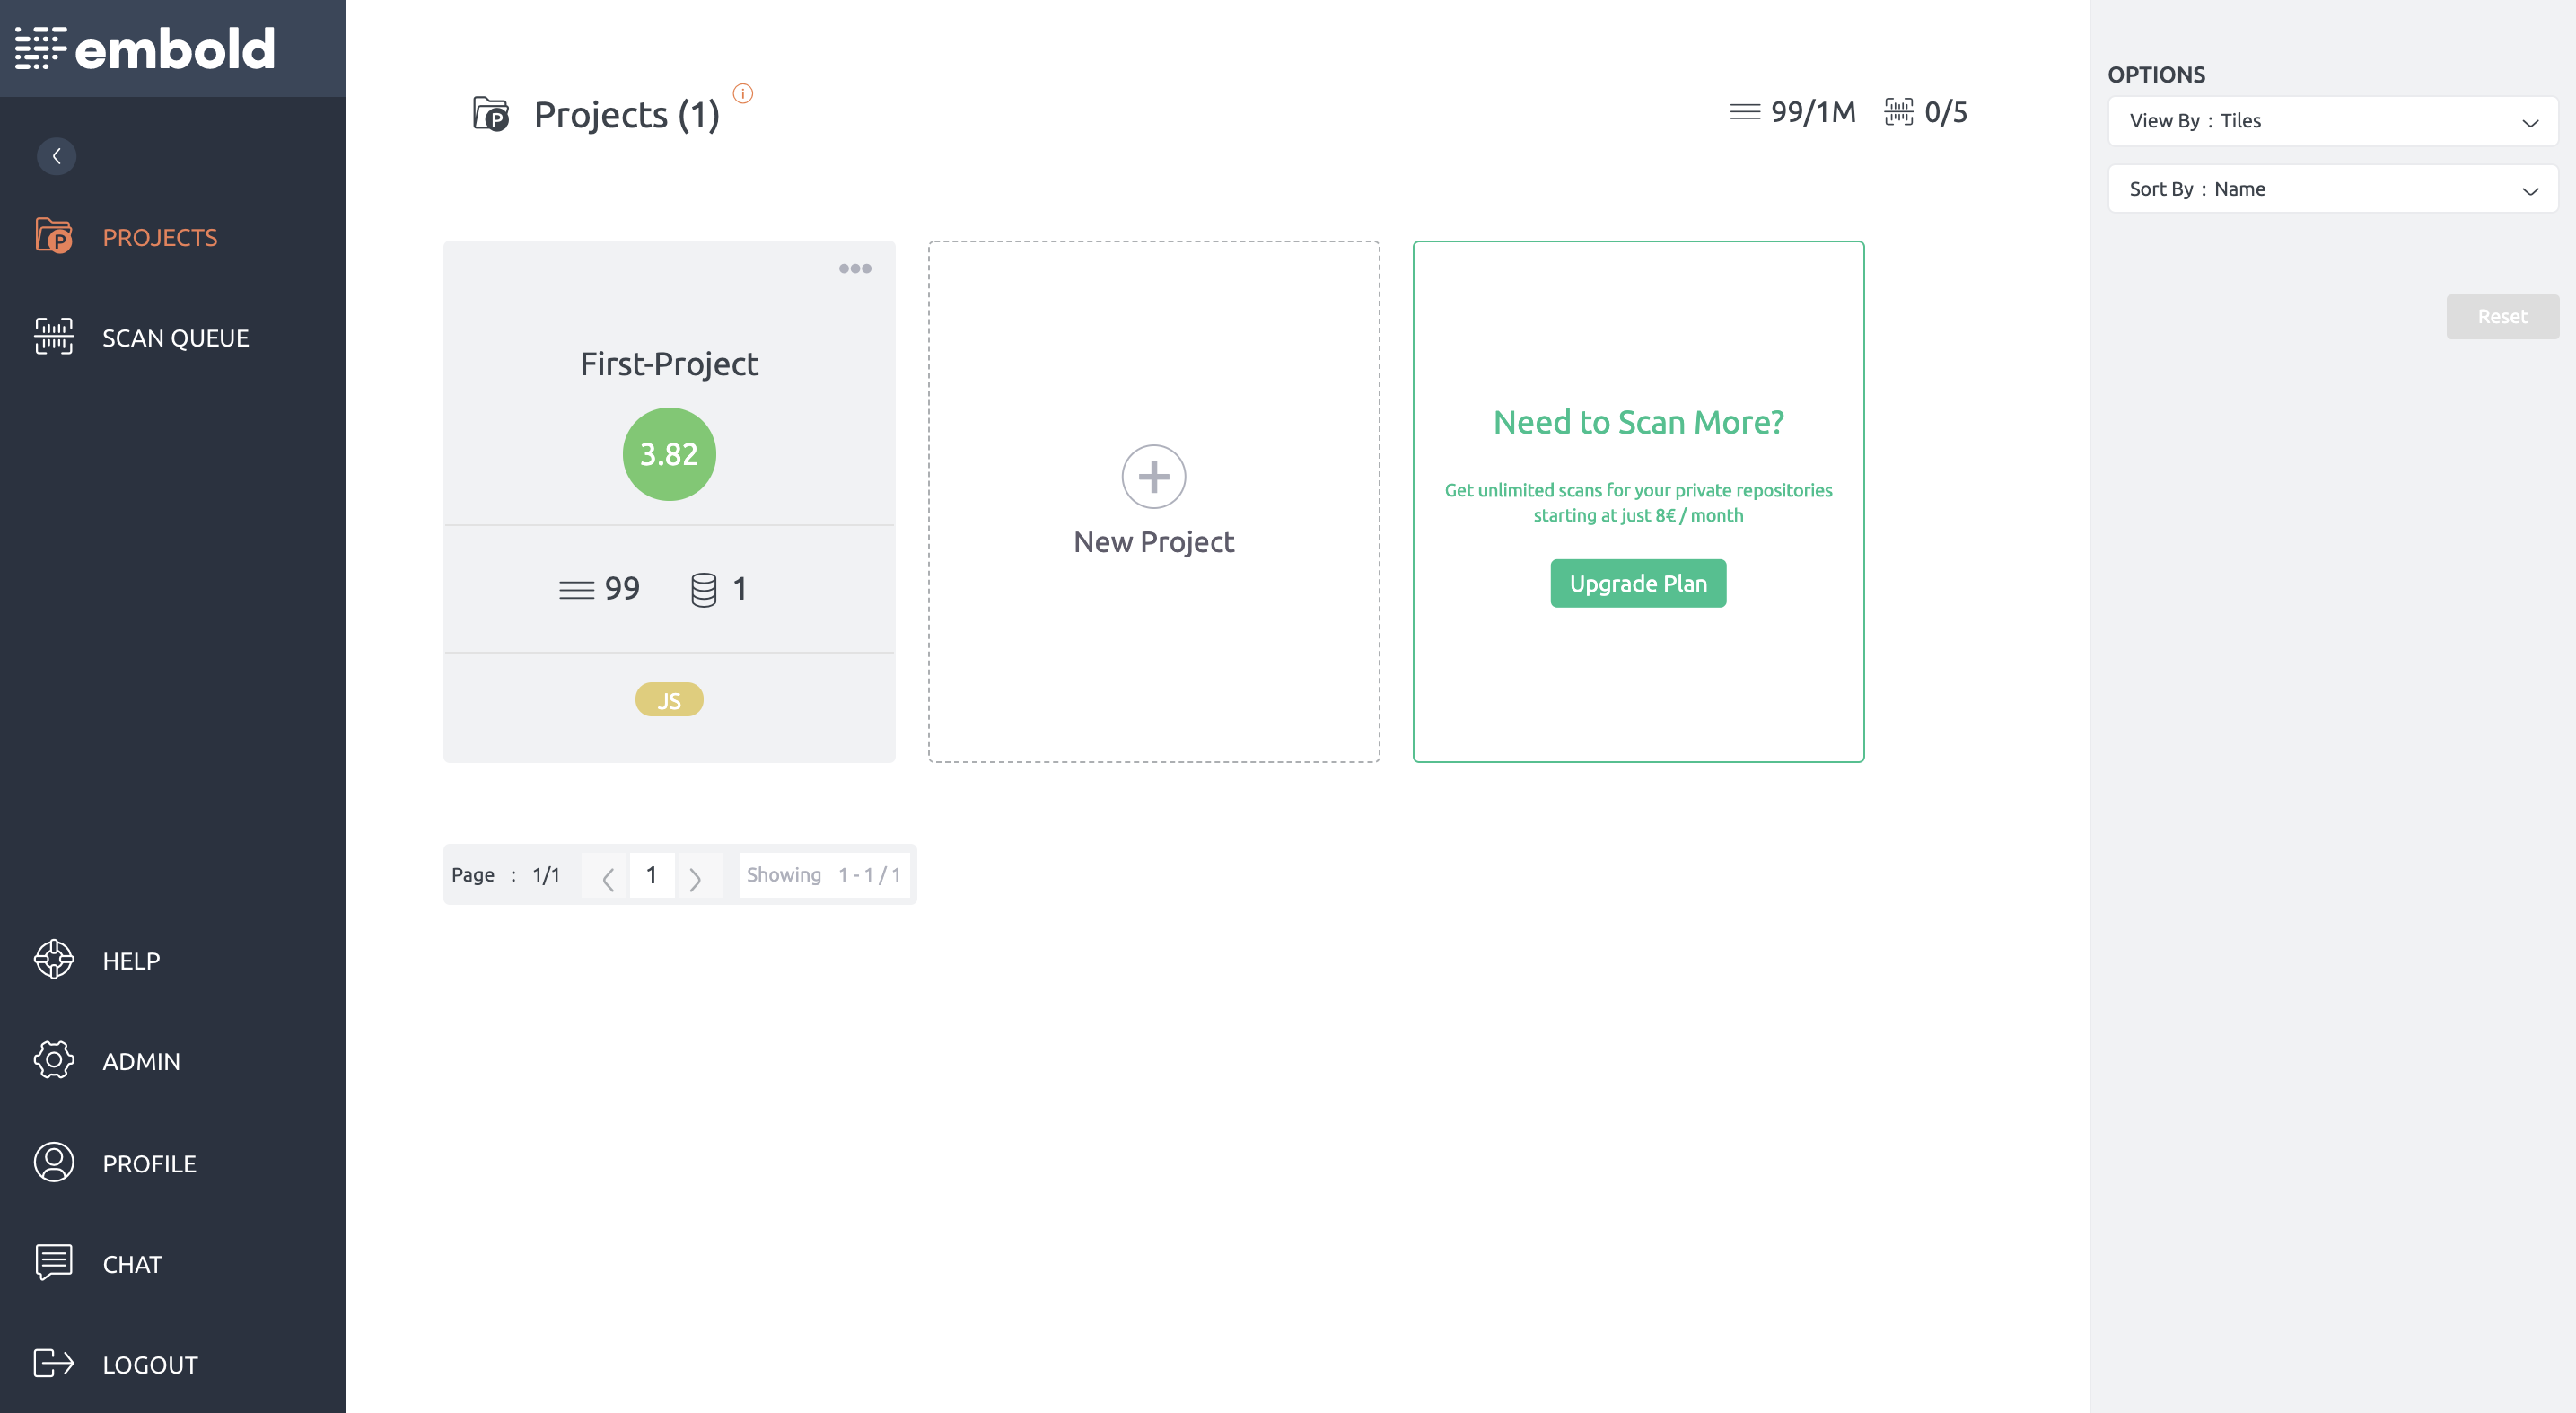
\includegraphics[width=6.5in, height=2.8in]{task-model.png}
\caption{Task Model ~\cite{emboldio}}
\label{fig:Task}
\end{center}
\end{figure}


\section{Scenarios}
The Embold is available as Open Source, Cloud and On Premise Self Hosted Environment. Various Pricing Plans are also available keeping in mind the need of the user. If somebody wants to use for once or just a few repositories it is free up-to 5 repositories but  all the repositories should be open source. \par
\begin{figure}[htbp]
\begin{center}
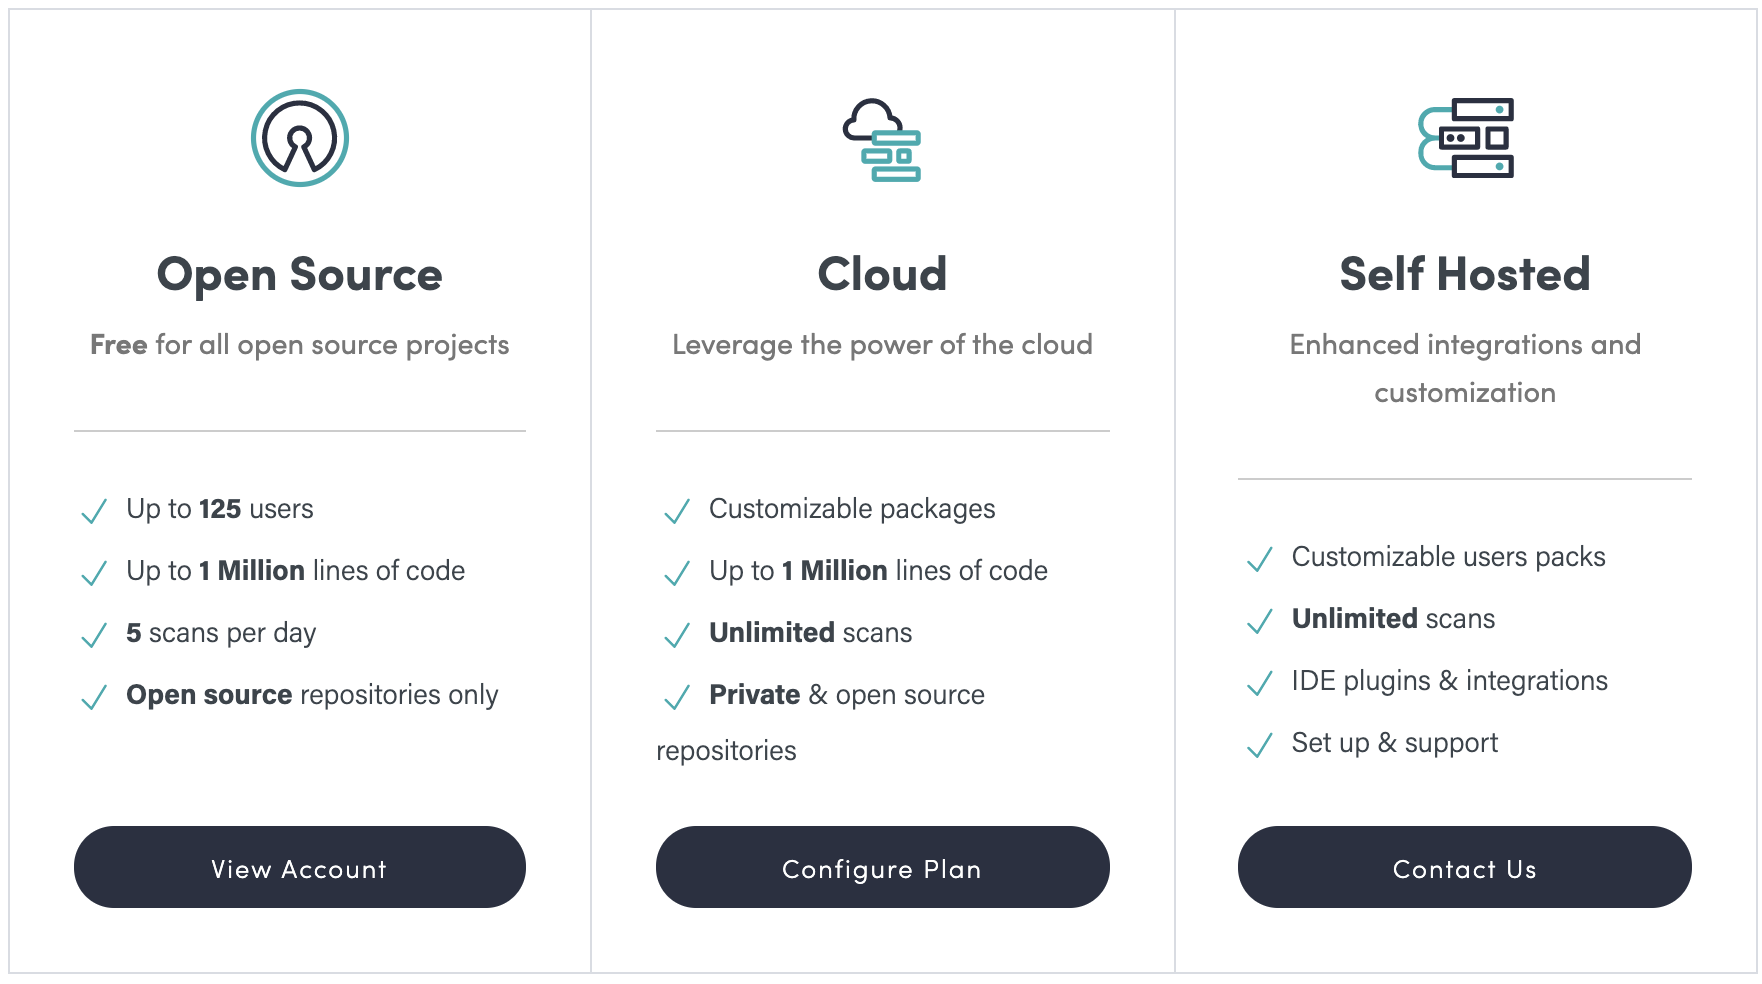
\includegraphics[width=6.5in, height=2.5in]{scenario.png}
\caption{Scenario ~\cite{emboldio}}
\label{fig:Scenario}
\end{center}
\end{figure}
\indent It has various price plans for the Start ups, Small Medium Enterprises and big Enterprises. As now world is moving towards the autonomous driving era, hence Automotive sector is using Embold eagerly, also few financial institutions are using Embold. The over view of the User Scenario is shown in Figure~\ref{fig:Scenario}.
\section{Persona}
I prepared a user persona of an Embold Developer as shown in the Figure~\ref{fig:User Persona}. As persona is just about an imaginary character, here Mr. Dane is the Software Engineer who has prepared the tool Embold. He has different and interesting programming skills as well as he has  comprehensive management and other soft skills. Hence he wants to develop a tradition to write the clean code so he very motivated and working to the Embold to new heights where all the user groups can perform their tasks very efficiently. Mr. Dane is also committed to   include more programming languages which can be analyzed using the Embold.
\begin{figure}[htbp]
\begin{center}
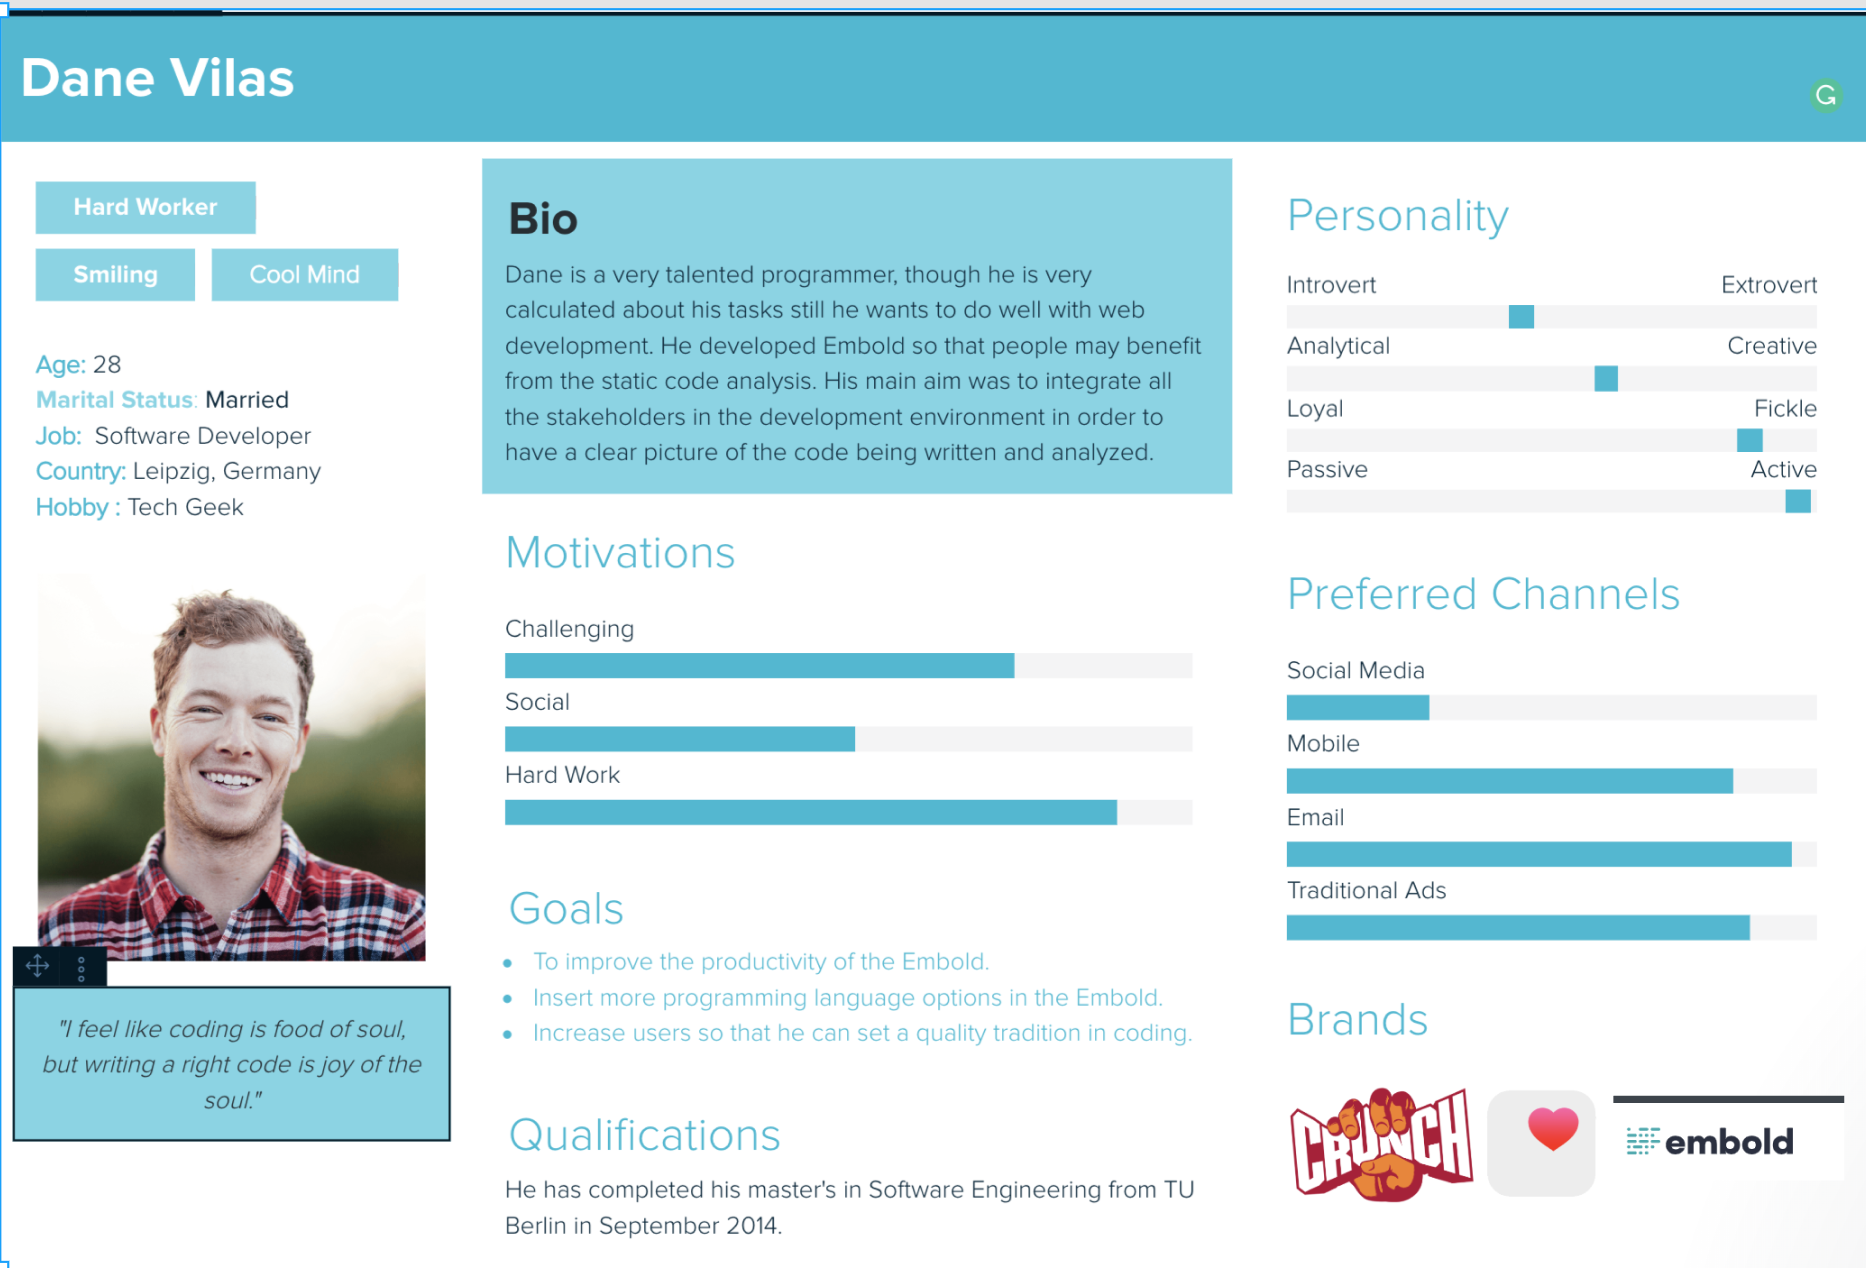
\includegraphics[width=6.5in, height=6in]{persona.png}
\caption{User Persona ~\cite{persona}}
\label{fig:User Persona}
\end{center}
\end{figure}